\section{(3.2)}
% Rinnai US has recently developed a new hydronic air handling unit (AHU Series 37AHA),
% designed for residential heating applications. In this system, hot water sourced from a
% tankless water heater will be circulated through a finned-tube heating coil, which is
% installed in the main branch of a ductwork system with dimensions of 20 in. x 18 in. A
% homeowner has calculated that a heating capacity of 96,000 Btu/hr is required to maintain
% the desired comfort conditions in their home. Air entering the ductwork will be at an initial
% temperature of 70°F, and it needs to be heated to 150°F before being distributed throughout
% the ductwork. The hot water supply to the heating coil will enter at a temperature of 180°F.
% Design a hot water heating coil for this application.
% Please fill in heat exchanger design data (with units) in the table below:
% HEAT EXCHANGER DESIGN DATASHEET
% TYPE
% SECTION: TUBE BANK
% WORKING FLUID
% VOLUME FLOW RATE
% INLET TEMPERATURE
% OUTLET TEMPERATURE
% PRESSURE DROP
% SECTION: TUBE
% TUBE MATERIAL
% WORKING FLUID
% VELOCITY
% TUBE INNER DIAMETER
% TUBE OUTER DIAMETER
% NUMBER OF TUBE ROWS
% NUMBER OF TUBES PER ROW
% TUBE SPACING (xt x xL)
% INLET TEMPERATURE
% OUTLET TEMPERATURE
% HEAD LOSS
% FIN MATERIAL
% FIN PITCH
% FIN THICKNESS
% HEADER SIZE
% HEAT EXCHANGER PARAMETERS
% THERMAL CAPACITY
% EFFECTIVENESS
% CAPACITY RATIO
% OVERALL HEAT TRANSFER COEFFICIENT
% NUMBER OF TRANSFER UNITS (NTU)
% HEAT EXCHANGER DIMENSIONS (LxHxW )

\textit{Rinnai US has recently developed a new hydronic air handling unit (AHU Series 37AHA), designed for residential heating applications. In this system, hot water sourced from a tankless water heater will be circulated through a finned-tube heating coil, which is installed in the main branch of a ductwork system with dimensions of 20 in. x 18 in. A homeowner has calculated that a heating capacity of 96,000 Btu/hr is required to maintain the desired comfort conditions in their home. Air entering the ductwork will be at an initial temperature of 70$^\circ$F, and it needs to be heated to 150$^\circ$F before being distributed throughout the ductwork. The hot water supply to the heating coil will enter at a temperature of 180$^\circ$F. Design a hot water heating coil for this application.}

\subsection{Assumptions:}
\begin{enumerate}
    \item Material chosen is type K copper for the pipe.
    \item From Table 2-1, an airflow of 500 fpm is used (can use 400-500 fpm for heating
          coils).
    \item Water flow velocity is 4 fps (this is due to the erosion limit of 6 fps and
          suction limit is 5 fps).
    \item Material chosen for the fins is copper.
    \item Let the outer diameter be 0.402 in (this is reasonable for finned-tube nex).
    \item From figure c.4a, $x_1 = 0.866$ in + $x_4 = 1.0$ in.
    \item Let the inner diameter be 0.305 in (from table A.6 using type K 1/4in NPS).
\end{enumerate}

\subsection{Sketch:}
Sketch will be shown after analysis.

\subsection{Analysis:}
Overall heat trsanfer for fine thinned tubes:
\begin{equation*}
    \frac{1}{U_{\text{FT}}} = \frac{1}{h_i \left(\frac{A_i}{A_{o}}\right)} + \frac{R_{fi}}{\left(\frac{A_i}{A_{o}}\right)} + R_{fo} + \frac{1}{h_o \eta_{so}}
\end{equation*}
from C.3: assuming distilled water above 122$^\circ$F and assuming compressed air,
\begin{align*}
    R_{fi} = 0.0011 \frac{\text{ft}^2 \cdot \text{hr} \cdot ^\circ \text{F}}{\text{Btu}}, \quad R_{o} = 0.00188 \frac{\text{ft}^2 \cdot \text{hr} \cdot ^\circ \text{F}}{\text{Btu}}
\end{align*}
\subsubsection{Heat Transfer Coeffiicent ($h_i$)}
\begin{align*}
    m_a c_{p, a} \Delta T_a = 96000 = m_w c_{p, w} \Delta T_w
\end{align*}
We assume that $m_a = m_w$. Then,
\begin{align*}
    \Delta T_a          & = T_{a, o} - T_{a, i} = 150 - 70 = 80^\circ F                           \\
    \implies \Delta T_w & = \Delta T_a \frac{c_{p, w}}{c_{p, a}} = 80 \frac{0.24}{1} = 20^\circ F \\
    \implies T_{w, o}   & = T_{w, i} - \Delta T_w = 180 - 20 = 160^\circ F                        \\
\end{align*}
Using $T_{w, \text{avg}} = 170^\circ F$, from Table A-9E:
\begin{align*}
    \rho = 60.78 \frac{\text{lb}}{\text{ft}^3}, \quad k = 0.386 \frac{\text{Btu}}{\text{hr} \cdot \text{ft} \cdot \text{R}}, \quad \mu = 2.483 \times 10^{-4} \frac{\text{lb}}{\text{ft} \cdot \text{s}}, \quad \text{Pr} = 2.80
\end{align*}
Find the Reynolds number:
\begin{align*}
    \text{Re}_{D_i} = \frac{\rho \bar{v} D_i}{\mu} = \frac{60.78 \cdot 4 \cdot 0.305}{2.483 \times 10^{-4}} = 24890.5
\end{align*}
This is fully turbulent flow. Also since $0.7 < \text{Pr} < 160$, we can use the Dittus-Boelter equation:
\begin{align*}
    \bar{h}_{i} & = 0.023 \cdot \frac{k}{D_i} \text{Re}_{D_i}^{0.8} \text{Pr}^{0.3} = 0.023 \cdot \frac{0.386}{0.305} \cdot \frac{12}{1} \cdot (24890)^{0.8} \cdot 2.9^{0.3} \\
                & = 1581 \frac{\text{Btu}}{\text{hr} \cdot \text{ft}^2 \cdot ^\circ F}
\end{align*}
\subsubsection{Finding $h_o$}
The average temperature is $T_{a, \text{avg}} = 110^\circ F$. From Table A-15E:
\begin{align*}
    \rho = 0.06963 \frac{\text{lb}}{\text{ft}^3}, \quad c_p = 0.240 \frac{\text{Btu}}{\text{lb} \cdot ^\circ F}, \quad k = 0.01552 \frac{\text{Btu}}{\text{hr} \cdot \text{ft} \cdot ^\circ F}, \quad \mu = 1.299 \times 10^{-5} \frac{\text{lb}}{\text{ft} \cdot \text{s}}, \quad \text{Pr} = 0.7245
\end{align*}
From Chart C.4a:
\begin{figure}[H]
    \centering
    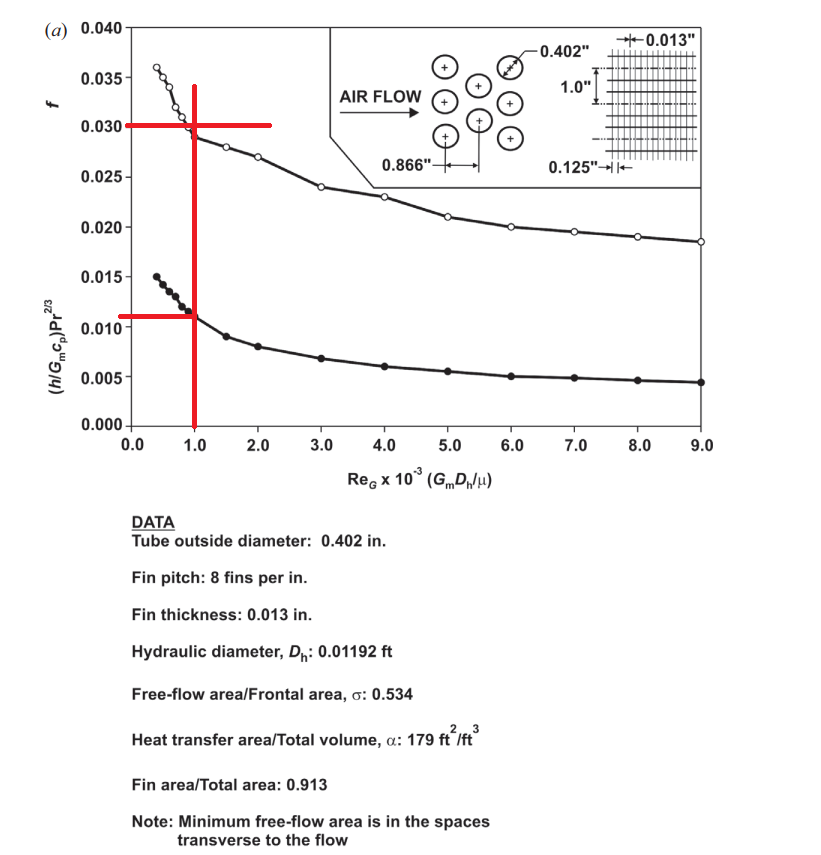
\includegraphics[width=0.9\textwidth]{Questions/Figures/Q1 Chart C4a.png}
    \caption{Chart C.4a}
    \label{fig:chartC4a}
\end{figure}
\begin{align*}
    G_m             & = \frac{\rho \bar{v}}{\sigma} = \frac{0.06963 \cdot 500}{0.534}\frac{1}{60} = 1.08 \frac{\text{lb}}{\text{ft}^2 \cdot \text{s}}                                                      \\
    \text{Re}_{G_m} & = \frac{G_m D}{\mu} = \frac{1.08 \cdot 0.01192}{1.299 \times 10^{-5}} = 987 \quad \therefore j\approx 0.011                                                                          \\
    \bar{h}_{o}     & = \frac{j G_m C_p}{\text{Pr}^{0.66}} = \frac{0.011 \cdot 1.09 \cdot 0.2405}{0.7245^{0.66}} \cdot \frac{3600}{1} = 12.9 \frac{\text{Btu}}{\text{hr} \cdot \text{ft}^2 \cdot ^\circ F}
\end{align*}
\subsubsection{Find $\phi$}
\begin{align*}
    \frac{A_i}{A_o}  & = \frac{A_{i} / \Omega}{A_{o} / \Omega} = \frac{\pi D_i}{x_t x_L} = \frac{\pi D_i}{\alpha x_t x_i} = \frac{\pi 0.305}{17.9 \cdot 1 \cdot 0.866} \cdot \frac{12}{1} = 0.0741 \\
    m                & = \sqrt{\frac{2 h_0}{h_\text{fin} t}} = \sqrt{\frac{2 \cdot 12.9}{232 \cdot 0.013 \cdot \frac{1}{12}}} = 10.1 \frac{1}{\text{ft}}                                           \\
    \Psi             & = \frac{M}{r} = \frac{x_t}{D_o} = \frac{1}{0.402} = 2.49                                                                                                                    \\
    L                & = \sqrt{\left(\frac{x_t}{2}\right)^2 + x_L^2} \cdot \frac{1}{2} = \sqrt{\left(\frac{1}{2}\right)^2 + 0.866^2} \cdot \frac{1}{2} = 0.5                                       \\
    M                & = \frac{x_t}{2} = \frac{1}{2} = 0.5                                                                                                                                         \\
    \beta            & = \frac{L}{M} = 1                                                                                                                                                           \\
    \frac{R_{eq}}{r} & = 1.27 \Psi \sqrt{\beta - 0.3} = 1.27 \cdot 2.49 \sqrt{1 - 0.3} = 2.65                                                                                                      \\
    \phi             & = \left(\frac{R_{eq}}{r} - 1\right)\left(1 + 0.35 \ln\left(\frac{R_{eq}}{r}\right)\right) = \left(2.65 - 1\right)\left(1 + 0.35 \ln(2.65)\right) = 2.21
\end{align*}
\subsubsection{Overal Heat Transfer Coefficient}
Fin efficiency:
\begin{align*}
    \eta_{o}  & = \frac{\tanh{mr\phi}}{mr\phi} = \frac{\tanh{10.1 \cdot 0.0168 \cdot 2.21}}{10.1 \cdot 0.0168 \cdot 2.21} = 0.956 \\
    \eta_{so} & = 1 - \frac{A_{\text{fin}}}{A} \left(1 - \eta_o \right) = 1 -  0.913 \left(1 - 0.956\right) = 0.96
\end{align*}
The overall heat transfer coefficient is:
\begin{align*}
    U_{FT} & = \left(\frac{1}{h_i \left(\frac{A_i}{A_o}\right)} + \frac{R_{fi}}{\left(\frac{A_i}{A_o}\right)} + R_{fo} + \frac{1}{h_o \eta_{so}}\right)^{-1} \\
           & = \left(\frac{1}{1581 \cdot 0.0741} + \frac{0.0011}{0.0741} + 0.00199 + \frac{1}{12.9 \cdot 0.96}\right)^{-1}                                   \\
           & = 9.43 \frac{\text{Btu}}{\text{hr} \cdot \text{ft}^2 \cdot ^\circ F}
\end{align*}

\subsubsection{Surface Area}
From the $\epsilon$-$NTU$ method:
\begin{equation*}
    A_o = \frac{c_\text{min} \text{NTU}}{U}
\end{equation*}
From heat balance for air:
\begin{align*}
    \dot{Q}      & = C_a (T_{a, o} - T_{a, i})                                                                                 \\
    \implies C_a & = \frac{\dot{Q}}{T_{a, o} - T_{a, i}} = \frac{96000}{80} = 1200 \frac{\text{Btu}}{\text{hr} \cdot ^\circ F} \\
\end{align*}
For water:
\begin{align*}
    C_w = C_h = C_c \frac{T_{a, o} - T_{a, i}}{T_{w, o} - T_{w, i}} = 1200 \frac{80}{20} = 4800 \frac{\text{Btu}}{\text{hr} \cdot ^\circ F}
\end{align*}
This confirms that $m_a = m_w$ and $c_{p, w}/c_{p, a} = 4$. Calculating effectivness:
\begin{align*}
    \epsilon & = \frac{C_c}{c_{\text{min}}} \left(\frac{T_{c, o} - T_{c, i}}{T_{h, o} - T_{h, i}}\right) = \frac{4800}{1200} \left(\frac{150 - 70}{180 - 160}\right) = 0.727
\end{align*}
Double checking $\dot{Q}$:
\begin{align*}
    \dot{Q} & = \epsilon c_\text{min} (T_{w_i} - T_{a_i}) 0.727 \cdot 1200 \cdot (180 - 70) \approx 96000 \text{Btu/hr}
\end{align*}

Determinign NTU from Figure 4.12:
\begin{figure}[H]
    \centering
    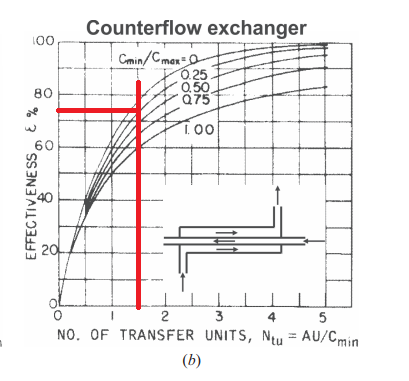
\includegraphics[width=0.9\textwidth]{Questions/Figures/Q1 Figure 4.12.png}
    \caption{Figure 4.12}
    \label{fig:figure4.12}
\end{figure}
\begin{align*}
    \text{NTU} & = 1.5 < 3, \quad \text{good}                                                          \\
    A_o        & = \frac{C_\text{min} \text{NTU}}{U} = \frac{1200 \cdot 1.5}{9.43} = 191.4 \text{ft}^2
\end{align*}
Total heat transfer volume:
\begin{align*}
    \Omega = \frac{A_o}{\alpha} = \frac{191}{179} = 1.07 \text{ft}^3
\end{align*}
Depth at heat exchanger:
\begin{align*}
    w = \frac{\Omega}{A_f} = \frac{1.07}{20 \cdot 18} \left(\frac{12}{1}\right)^2 = 5.18 \text{in} \approx = 6 \text{in}
\end{align*}
Number of tube rows:
\begin{align*}
    N_r & = \frac{w}{x_L} = \frac{5.18}{0.866} = 5.9 \approx 6 \text{ rows}
\end{align*}
Number of tubes per row:
\begin{align*}
    A_\text{tube} & = N_\text{tube} \frac{\pi D_i^2}{4} \quad \therefore N_\text{tube} = \frac{4 A_\text{tube}}{\pi D_i^2} \\
\end{align*}
since
\begin{align*}
    \dot{m}_w & = \rho_w \bar{v}_w A_\text{tube}, \quad c_h = \dot{m}_w c_{p, w}
\end{align*}
then,
\begin{align*}
    N_{\text{tube}} & = \frac{4 C_h}{c_{p, w} \bar{v}_w \pi D_i^2}                                                                                \\
                    & = \frac{4 \cdot 4800}{1 \cdot 60.79 \cdot 4 \cdot \pi \cdot 0.305^2} \cdot \left(\frac{12}{1}\right)^2 \cdot \frac{1}{3600} \\ &
                    & = 10.4 \approx 11 \text{ tubes}
\end{align*}
Heigh of heating cool: 
\begin{align*}
H = N_\text{tube} x_t = 10.4 \cdot 1 \approx 11 \text{ in}
\end{align*}
Length of the heat exchanger:
\begin{align*}
    L & = \frac{A_f}{H} = \frac{20 \cdot 18}{10.4} \cdot \left(\frac{1}{12}\right)^2 = 34.6 \approx 35 \text{ ft}
\end{align*}
Main header diameter:
\begin{align*}
Q_w &= A_\text{header} v_w = N_\text{tube} \cdot \frac{\pi D_i^2}{4} \cdot v_w \\
\implies D_\text{header} &= \sqrt{N_\text{tube}} D_i = \sqrt{11} (0.305) = 1 \text{ in} 
\end{align*}
Airflow rate:
\begin{align*}
Q_a &= v_a A_f = 500 \cdot 20 \cdot 18 \cdot \left(\frac{1}{12}\right)^2 = 1250 \text{cfm} 
\end{align*}
Pressure loss for air across tubes:
\begin{align*}
\Delta P_\text{bank} &= \frac{G_m^2}{2 P_{a, i}}\left[(1 + \sigma^2) \left(\frac{P_{a, i}}{P_{a, o}} - 1\right) + f\frac{A_{T}}{A_c}\frac{\rho_a, i}{\rho_\text{mean}}\right]
\end{align*}
Area:
\begin{align*}
\frac{A_T}{A_c} = \frac{4w}{D_h} = \frac{4 \cdot 5.4}{0.01192} \left(\frac{1}{12}\right) = 151
\end{align*}
mean density:
\begin{align*}
\rho_{\text{mean}} &= \frac{\rho_{a, i} + \rho_{a, o}}{2} = \frac{0.07489 + 0.06507}{2} = 0.06998 \text{lb/ft}^3
\end{align*}
Then,
\begin{align*}
\Delta P_\text{bank} &= \frac{1.08^2}{2 \cdot 0.07489} \left[(1 + 0.534^2) \left(\frac{0.07489}{0.06507} - 1\right) + 0.003 \cdot 151 \cdot \frac{0.07489}{0.06998}\right] \\
&= 0.22 \text{ in wg}
\end{align*}
From Moody diagram:
\begin{figure}[H]
    \centering
    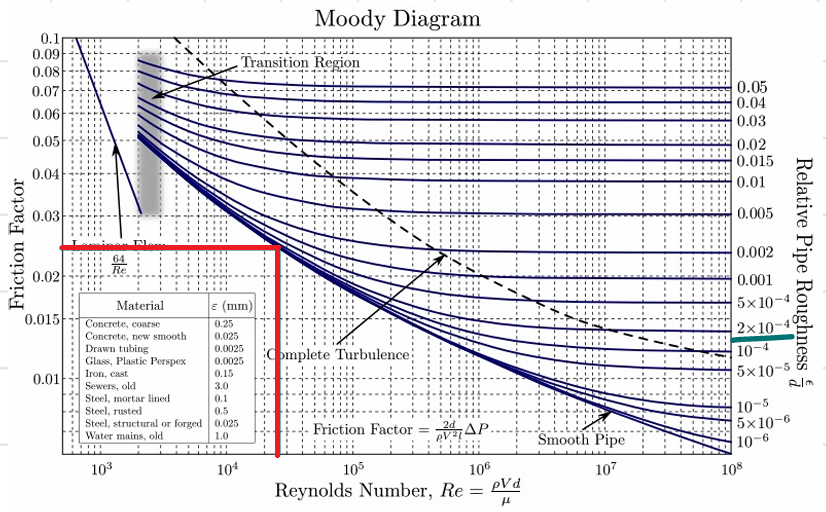
\includegraphics[width=0.9\textwidth]{Questions/Figures/Q1 Moody Diagram.png}
    \caption{Moody Diagram}
    \label{fig:moodyDiagram}
\end{figure}
\begin{align*}
    f &= 0.026 \\
    L_\text{tube} = 6 \cdot 35 = 210 \text{ in} \\
    \text{minor loss} k &= 2 \\
    H_{1T} &= \left(f \frac{L_\text{tube}}{D_i} + k\right) \frac{\bar{v}_w^2}{2g} = \left(0.026 \cdot \frac{210}{0.305} + 5 \cdot 2\right) \frac{4^2}{2 \cdot 32.2} \\
    &= 7 \text{ ft wg}
\end{align*}
\subsection{Drawing}
\begin{figure}[H]
    \centering
    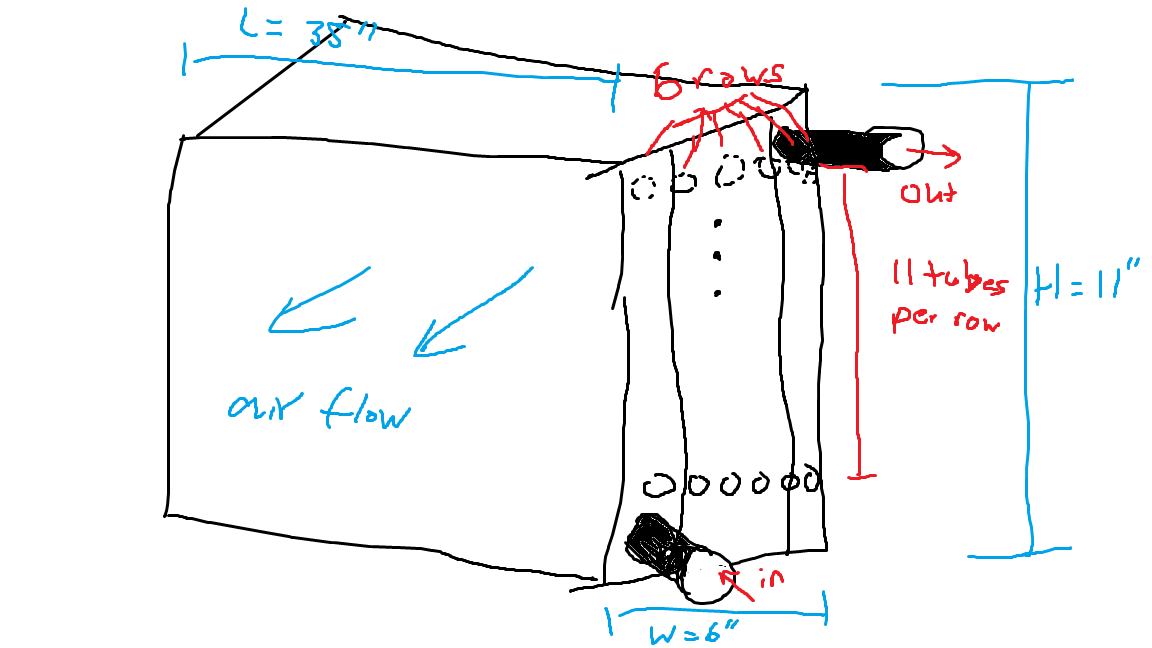
\includegraphics[width=0.9\textwidth]{Questions/Figures/Q1 Drawing.png}
    \caption{Drawing}
    \label{fig:drawing}
\end{figure}
\subsection{Conclusion}
In response to the heating requirements for the residential application, a hot water heating coil was successfully designed for the Rinnai US AHU Series 37AHA system. The unit was designed with finned-tube coils to efficiently heat the air, achieving the necessary 96,000 Btu/hr heating capacity.

To accommodate the specific dimensions of the ductwork (20 in. x 18 in.), the hexagonal coil with dimensions of 35 in. x 11 in. x 6 in. was selected. This design ensures that the heating coil can effectively integrate into the system while meeting the necessary air heating capacity.

A transition fitting will be required to connect the coil to the duct, ensuring compatibility between the coil size and the existing air handling system. This fitting will allow for a smooth connection between the hexagonal coil and the rectangular ductwork.

The hot water supply entering the coil at 180$^\circ$F will be sufficient to raise the air temperature from 70$^\circ$F to 150$^\circ$F, effectively maintaining the desired comfort conditions in the home. The temperature differential is within the system's operational range, ensuring that the unit functions efficiently.

All design specifications and relevant data from the unit's datasheet are provided on the following page, confirming that the heating coil will meet the system's performance requirements. This design will provide reliable and consistent heating for the residential space, meeting both the homeowner's and the system's needs.

\subsubsection{Data Sheet}
\begin{longtable}[c]{lc}
    \caption{HEAT EXCHANGER DESIGN DATASHEET} \\
    
    \toprule
    \multicolumn{2}{c}{\textbf{HEAT EXCHANGER DESIGN DATASHEET}} \\
    \midrule
    \textbf{TYPE} &  \\
    \midrule
    \textbf{SECTION: TUBE BANK} &  \\
    \midrule
    WORKING FLUID &  Air\\
    VOLUME FLOW RATE &  1250 cfm \\
    INLET TEMPERATURE &  70$^\circ$F\\
    OUTLET TEMPERATURE &  150$^\circ$F\\
    PRESSURE DROP &  0.22 in wg \\
    \midrule
    \textbf{SECTION: TUBE} &  \\
    \midrule
    TUBE MATERIAL &  Copper \\
    WORKING FLUID &  Water \\
    VELOCITY &  4 fps \\
    TUBE INNER DIAMETER &  0.305 in \\
    TUBE OUTER DIAMETER &  0.402 in \\
    NUMBER OF TUBE ROWS &  6 \\
    NUMBER OF TUBES PER ROW &  11 \\
    TUBE SPACING (xt x xL) &  1 in x 0.866 in \\
    INLET TEMPERATURE &  180$^\circ$F\\
    OUTLET TEMPERATURE &  160$^\circ$F\\
    HEAD LOSS &  7 ft wg \\
    FIN MATERIAL &  Copper \\
    FIN PITCH &  8 fins/in \\
    FIN THICKNESS &  0.013 in \\
    HEADER SIZE &  1 in \\
    \midrule
    \textbf{HEAT EXCHANGER PARAMETERS} &  \\
    \midrule
    THERMAL CAPACITY &  96 000 Btu/hr \\
    EFFECTIVENESS &  0.727 \\
    CAPACITY RATIO &  0.25 \\
    OVERALL HEAT TRANSFER COEFFICIENT &  9.43 Btu/hr ft$^2$ $^\circ$F \\
    NUMBER OF TRANSFER UNITS (NTU) &  1.5 \\
    \textbf{HEAT EXCHANGER DIMENSIONS (LxHxW)} &  35 in x 11 in x 6 in \\
    \bottomrule
    \end{longtable}
% \begin{table}[H]
% \centering
% \begin{tabular}{cc}
% \toprule
% \multicolumn{2}{c}{\textbf{HEAT EXCHANGER DESIGN DATASHEET}} \\
% \midrule
% \textbf{TYPE} &  \\
% \textbf{SECTION: TUBE BANK} &  \\
% WORKING FLUID &  Air\\
% VOLUME FLOW RATE &  1250 cfm \\
% INLET TEMPERATURE &  70$^\circ$F\\
% OUTLET TEMPERATURE &  150$^\circ$F\\
% PRESSURE DROP &  0.22 in wg \\
% \textbf{SECTION: TUBE} &  \\
% TUBE MATERIAL &  Copper \\
% WORKING FLUID &  Water \\
% VELOCITY &  4 fps \\
% TUBE INNER DIAMETER &  0.305 in \\
% TUBE OUTER DIAMETER &  0.402 in \\
% NUMBER OF TUBE ROWS &  6 \\
% NUMBER OF TUBES PER ROW &  11 \\
% TUBE SPACING (xt x xL) &  1 in x 0.866 in \\
% INLET TEMPERATURE &  180$^\circ$F\\
% OUTLET TEMPERATURE &  160$^\circ$F\\
% HEAD LOSS &  7 ft wg \\
% FIN MATERIAL &  Copper \\
% FIN PITCH &  8 fins/in \\
% FIN THICKNESS &  0.013 in \\
% HEADER SIZE &  1 in \\
% \textbf{HEAT EXCHANGER PARAMETERS} &  \\
% THERMAL CAPACITY &  96 000 Btu/hr \\
% EFFECTIVENESS &  0.727 \\
% CAPACITY RATIO &  0.25 \\
% OVERALL HEAT TRANSFER COEFFICIENT &  9.43 Btu/hr ft$^2$ $^\circ$F \\
% NUMBER OF TRANSFER UNITS (NTU) &  1.5 \\
% \textbf{HEAT EXCHANGER DIMENSIONS (LxHxW)} &  35 in x 11 in x 6 in \\
% \bottomrule
% \end{tabular}
% \end{table}